\chapter{分岐解析}
\indent 細胞内には転写制御、シグナル伝達、代謝といった分子間相互作用ネッ
トワークが存在します。こうしたネットワークの動態を理論的に追究するため
の手段として、数理生物学やシステム生物学の分野では連立微分方程式モデル
が用いられています。\\
\indent 連立微分方程式の解は連続値となるのが一般的です。しかし、式中の定数の値を増減させると、それまで定常状態にあった系がある値を境に、突如として振動を始めるなど、系の挙動が不連続的に変化することがあります。このような現象は非線形力学系の分野で研究されており、分岐(bifurcation)と呼ばれています。\\
\indent 連続の微分方程式からなぜこのような不連続な現象が生じるのでしょ
うか?本章では、この問いに答える能力を培うため、代表的な分岐であ
るSaddle-Node分岐、Hopf分岐、Pitchfork分岐を生物学的な実例とともに取り
上げます。

\section{Saddle-Node(サドル・ノード)分岐}
\subsection{Griffithモデル: 非線形力学系理論と双安定性(bistability)}
細胞内には、あたかもスイッチのON/OFFかのように、2つの安定状態を持つ系が
存在します。このような性質を「双安定性(bistability)」と呼び、力学系の理
論では安定固定点(Stable nodeまたはStable spiral)が2つ存在する状態として
説明されます。ここでは双安定性を示す系の例として、Griffithによって提案
された、自己フィードバック・ループを持つ遺伝子発現系のモデルを次に示し
ます。このモデルでは遺伝子XからmRNAが転写され、そのmRNAから翻訳されたタ
ンパク質が遺伝子X自体の転写を活性化します。Griffithはこれを次のようにモ
デル化しました(ただし、\(x\)はタンパク質、\(y\)はmRNAの存在量)。

\begin{figure}[ht]
        \centering 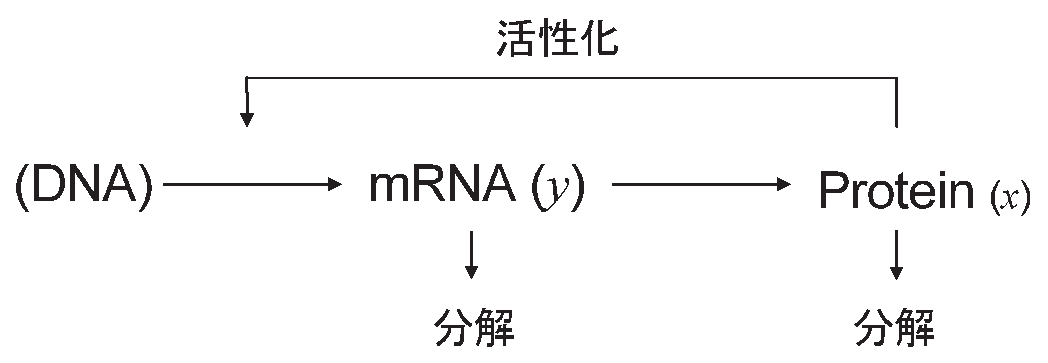
\includegraphics[height=2cm]{../Bifurcation/img/griffith_model.eps}
        \caption{Griffithモデル。翻訳されたタンパク質は自身をコードする遺伝子の転写を活性化する。}
        \label{fig:04sysbio} \end{figure}

\[
\left\{
\begin{array}{lclclll}
\dot x & = & -ax + y\\
\dot y & = & \displaystyle\frac{x^2}{1+x^2} - by\\
\end{array}
\right.\]

Griffithモデルはパラメータ\(a\)、\(b\)の値によってSaddleとNodeの個数が変わるSaddle-Node分岐を示します。

\subsection{相平面とヌルクライン}
\paragraph{相平面(phase plane)}
時間とともに変化する変数を縦軸・横軸にそれぞれ取った平面のこと。例えばGriffithモデルの相平面は、mRNA(\(y\))、Protein(\(x\))をそれぞれ縦軸・横軸に取った座標空間です。

\paragraph{ヌルクライン(nullcline)} 一般に、時間変化する量についての微分方程式が0と等しくなるような点の集合をヌルクライン(nullcline)と呼びます。
相平面上に描いたヌルクラインは図\ref{fig:05sysbio}のようになります。2変数系の場合、2つのヌルクラインの交点に
おいては系が定常状態になります。非線形力学系の分野では固定点(fixed point)と呼ばれます。

\paragraph{演習1:  Griffithモデルの相平面とヌルクライン}
Griffith モデルのヌルクラインを相平面上に描きなさい。

\subsection{ベクトル場}
\paragraph{ベクトル場(vector field)}
化学反応系が相平面上の一点で表される状態にあるとき、微小時間後にその点がどの方向に動くかをベクトルで示したもの。
描き方は次の通りです。

\[
\left\{
\begin{array}{lclclll}
\dot x & = & f(x,y)\\
\dot y & = & g(x,y)\\
\end{array}
\right.\]

という2変数の系があるとき、点\((x,y)\)に大きさ\((\dot x , \dot y)\)のベクトルを描きます。
下記のような具体例を考えましょう。

\[
\left\{
\begin{array}{lclclll}
\dot x & = & -x + 2y + x^2y\\
\dot y & = & 8 -2y -x^2y\\
\end{array}
\right.\]

この系において、点\((x,y)=(1,2)\)におけるベクトルを求めてみましょう。\((x,y)=(1,2)\)を
この微分方程式に代入すると、\((\dot x, \dot y)=(5,2)\)となります。これより、\(x\)方向に5、\(y\)方向
に2の大きさを持つベクトルを点(1,2)を原点として描けばよいことになります。\\

\indent ヌルクラインの定義より、\(x\)のヌルクライン上ではベクトルは垂直(\(\dot x = 0\))になります(図\ref{fig:05sysbio})。。

\begin{figure}[ht]
        \centering 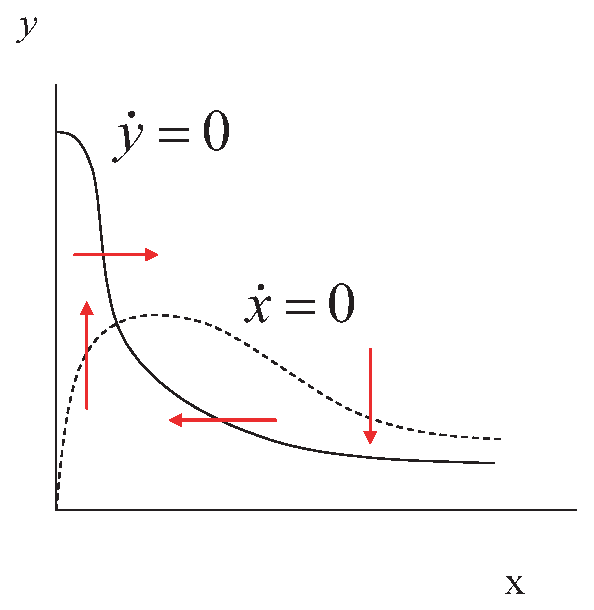
\includegraphics[height=6cm]{../Bifurcation/img/vectorfield.eps}
        \caption{相平面上に描いたヌルクラインとベクトル場}
        \label{fig:05sysbio} \end{figure}


\paragraph{演習2:  Griffithモデルのベクトル場}
「演習1」の結果にベクトル場の概略を描き加えなさい。


\subsection{線形化とヤコビ行列}
\paragraph{線形化(linearization)}
非線形の微分方程式を固定点の近傍でテイラー展開し、1次の項のみ残して2次以降の項を消去すること。

\paragraph{ヤコビ行列(Jacobian matrix)}
線形化を行った結果得られた1次項からなる正方行列のこと。線形化の手順は次の通りです。
\[
\left\{
\begin{array}{lclclll}
\displaystyle\frac{d}{dt}x_1 & = & F_1(x_1, \cdots , x_n)\\
                & \vdots & \\
\displaystyle\frac{d}{dt}x_n & = & F_n(x_1, \cdots , x_n)\\
\end{array}
\right.
\]

のような連立常微分方程式を固定点\(x_{k(fp)}\)の近傍でテイラー展開すると、

\[
\begin{array}{ccl}
\displaystyle\frac{d}{dt}
\left(
\begin{array}{c}
x_{1(fp)}+\Delta x_1\\
\vdots \\
x_{n(fp)}+\Delta x_n\\
\end{array}
\right)
& = &
\left(
\begin{array}{c}
F_{1(fp)}(x_1, \cdots , x_n)\\
\vdots \\
F_{n(fp)}(x_1, \cdots , x_n)\\
\end{array}
\right)

+

\left(
\begin{array}{ccc}
\frac{\partial F_1}{\partial x_1} & \cdots & \frac{\partial F_1}{\partial x_n} \\
\vdots                            &        & \vdots\\
\frac{\partial F_n}{\partial x_1} & \cdots & \frac{\partial F_n}{\partial x_n} \\
\end{array}
\right)
\left(
\begin{array}{c}
\Delta x_1\\
\vdots \\
\Delta x_n\\
\end{array}
\right)\\

&
+
&
\displaystyle\frac{1}{2}
\left( \Delta x_1 , \cdots , \Delta x_n \right)
\left(
\begin{array}{ccc}
\frac{\partial^2 F_1}{\partial x_1^2} & \cdots & \frac{\partial^2 F_1}{\partial x_1 \partial x_n} \\
\vdots                            &    \ddots    & \vdots\\
\frac{\partial^2 F_n}{\partial x_n \partial x_1} & \cdots & \frac{\partial^2 F_n}{\partial x_n^2} \\
\end{array}
\right)
\left(
\begin{array}{c}
\Delta x_1\\
\vdots \\
\Delta x_n\\
\end{array}
\right)\\

\end{array}
\]

を得ます(3次項以降省略)。このうち、固定点の定義より\(F_k(x_{1(fp)}, \cdots , x_{n(fp)})=0\)なので0次の項は
無視できます。また、2次の項\((\Delta x_{k(fp)})^2\)は微小量の2乗ですから、固定点近傍においては2次の項を近似的に0とみなして無視することができます。
よって下記のような式が得られます。

\[
\frac{d}{dt}
\left(
\begin{array}{c}
\Delta x_1\\
\vdots \\
\Delta x_n\\
\end{array}
\right)
=
\left(
\begin{array}{ccc}
\frac{\partial F_1}{\partial x_1} & \cdots & \frac{\partial F_1}{\partial x_n} \\
\vdots                            &        & \vdots\\
\frac{\partial F_n}{\partial x_1} & \cdots & \frac{\partial F_n}{\partial x_n} \\
\end{array}
\right)
\left(
\begin{array}{c}
\Delta x_1\\
\vdots \\
\Delta x_n\\
\end{array}
\right)\\
\]

ベクトル表記にすると、

\[ \frac{d}{dt}\Delta {\bf x} = {\bf J}\Delta {\bf x}\]

右辺に残った1階偏微分からなる行列{\bf J}をヤコビ行列と呼びます。


\paragraph{演習3:  Griffithモデルの線形化とヤコビ行列}
Griffith モデルを線形化し、ヤコビ行列を求めなさい。

\subsection{ヤコビ行列の固有値と安定性}
\paragraph{行列指数関数(matrix exponential)}
線形化した連立微分方程式の解となる関数です。上で得た微分方程式

\[ \frac{d}{dt}\Delta {\bf x} = {\bf J}\Delta {\bf x}\]

の解は下記のようになります。

\[\Delta {\bf x}=\exp({\bf J}t)\Delta {\bf x}_0\]

ただし、

\[\exp({\bf J}t) = {\bf I} + \frac{{\bf J}t}{1!} + \frac{{\bf J}^2 t^2}{2!} + \frac{{\bf J}^3 t^3}{3!} + \cdots\]

であり、\(\Delta {\bf x}_0\)は系に与えられた摂動の大きさ(固定点からのずれの初期値)です。

\paragraph{固有値(eigenvalue)}
行列指数関数は後々扱いが面倒なので、ヤコビ行列{\bf J}の固有値\(\lambda\)・固有ベクトル{\bf v}を用いて普通の指数関数に書き直しておきます。

\begin{eqnarray*}
\exp({\bf J}t){\bf v} & = & \left({\bf I} + \frac{{\bf J}t}{1!} + \frac{{\bf J}^2 t^2}{2!} + \frac{{\bf J}^3 t^3}{3!} + \cdots \right){\bf v}\\
                      & = & \left(1 + \frac{\lambda t}{1!} + \frac{\lambda^2 t^2}{2!} + \frac{\lambda^3 t^3}{3!} + \cdots \right){\bf v}\\
                      & = & \exp(\lambda t) {\bf v}\\
\end{eqnarray*}

また、初期摂動\(\Delta {\bf x}_0\)も固有ベクトルの線形結合として下のように表せます。

\[\Delta {\bf x}_0 = c_1 {\bf v}_1 + \cdots c_n {\bf v}_n \]

幾何学的な描像を図\ref{fig:06sysbio}に示しました。

\begin{figure}[ht]
        \centering 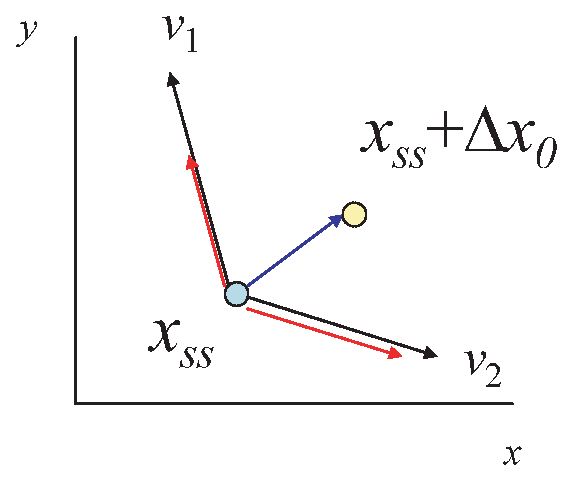
\includegraphics[height=6cm]{../Bifurcation/img/decomposition.eps}
        \caption{摂動(定常状態\(x_{ss}\)からのずれ)は固有ベクトルの線形結合として表せる。}
        \label{fig:06sysbio} \end{figure}


よって、固定点からのずれ\(\Delta {\bf x}\)は、

\begin{eqnarray*}
\Delta {\bf x}(t) & = & \exp({\bf J}t)\Delta {\bf x}_0\\
                 & = & \exp({\bf J}t)(c_1 {\bf v}_1 + \cdots c_n {\bf v}_n) \\
                 & = & c_1 \exp(\lambda_1 t){\bf v}_1 + \cdots c_n \exp(\lambda_n t){\bf v}_n \\
\end{eqnarray*}

となり、固有値が正の時には\(\Delta {\bf x}\)が発散し、負の時には収束する(すなわち固定点に戻る)ことがわかります(図\ref{fig:07sysbio})。

\begin{figure}[ht]
        \centering 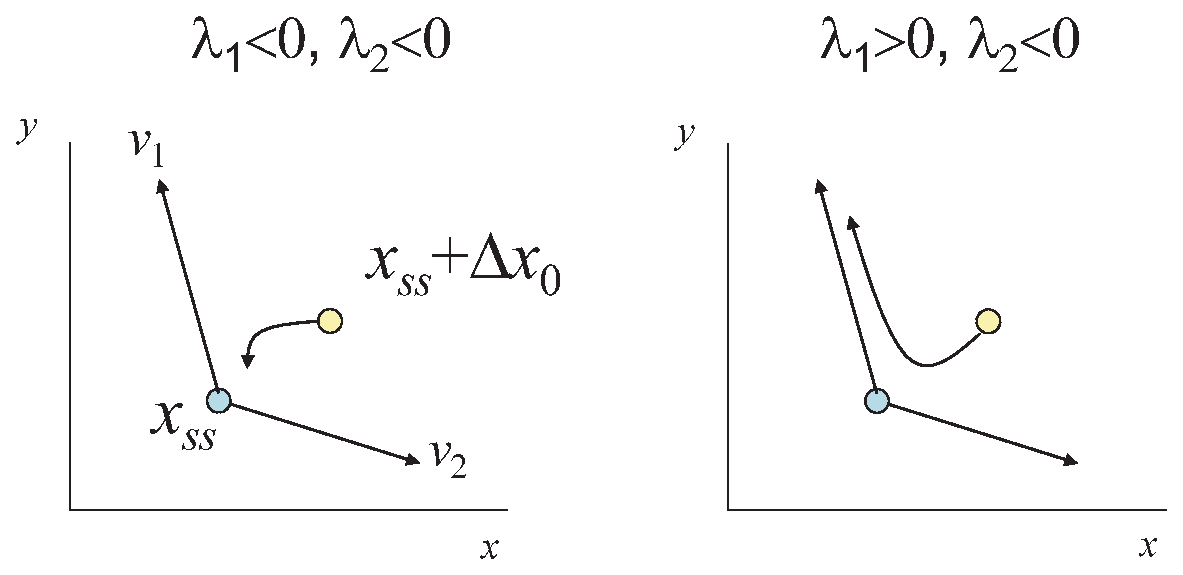
\includegraphics[height=5cm]{../Bifurcation/img/eigenvector.eps}
        \caption{(左)固有値がすべて負なら解軌跡は固定点に収束する。(右)正の固有値を含む固定点では解軌跡が発散する。}
        \label{fig:07sysbio} \end{figure}


\paragraph{固定点の分類} ヤコビ行列の固有値の正負・虚実の組み合わせにより、固定点は下表のように分類されます。注目している化学反応系の固定点がどのタイプにあたるのかを調べることで、化学反応系の動態を定性的に把握できます(図\ref{fig:08asysbio}、 \ref{fig:08bsysbio})。\\

\begin{center}
表: 固有値による固定点の分類\\
\begin{tabular}{clll}
\hline
固有値の虚実 & 固有値の符号       & 固定点の名称 & 時系列の特徴 \\
\hline
実数  & すべて正         & Unstable node  & 不安定な定常状態\\
   & すべて負         & Stable node    & 安定した定常状態\\
      & 正負混在         & Saddle         & 不安定な定常状態\\
\hline
複素数 & 実部がすべて負  & Stable spiral  & 減衰振動(安定解)\\
    & 正の実部を持つ  & Unstable spiral & 発散振動(不安定解)\\
       & 純虚数          & Center          & 調和振動\\
\hline
\end{tabular}
\end{center}

\begin{figure}[ht]
        \centering 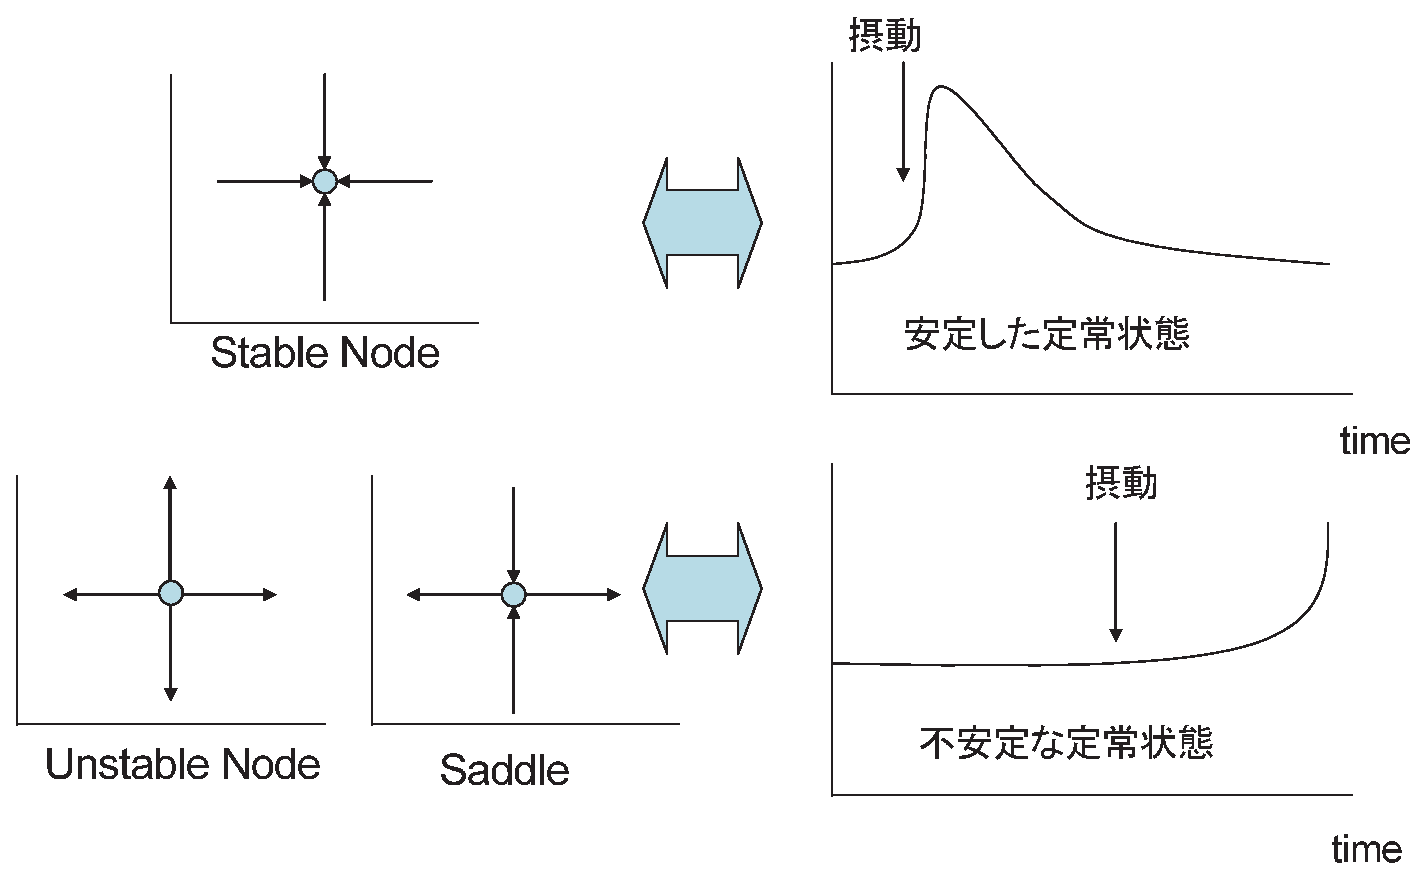
\includegraphics[height=6cm]{../Bifurcation/img/node_stability.eps}
                \caption{実数固有値のみの場合の固定点の分類。(左)それぞれの固定点近傍におけるベクトル場の特徴。正の固有値を1つでも含むと不安定な定常状態となる。(右)時系列の特徴。}
        \label{fig:08asysbio} \end{figure}
        
\begin{figure}[ht]
        \centering 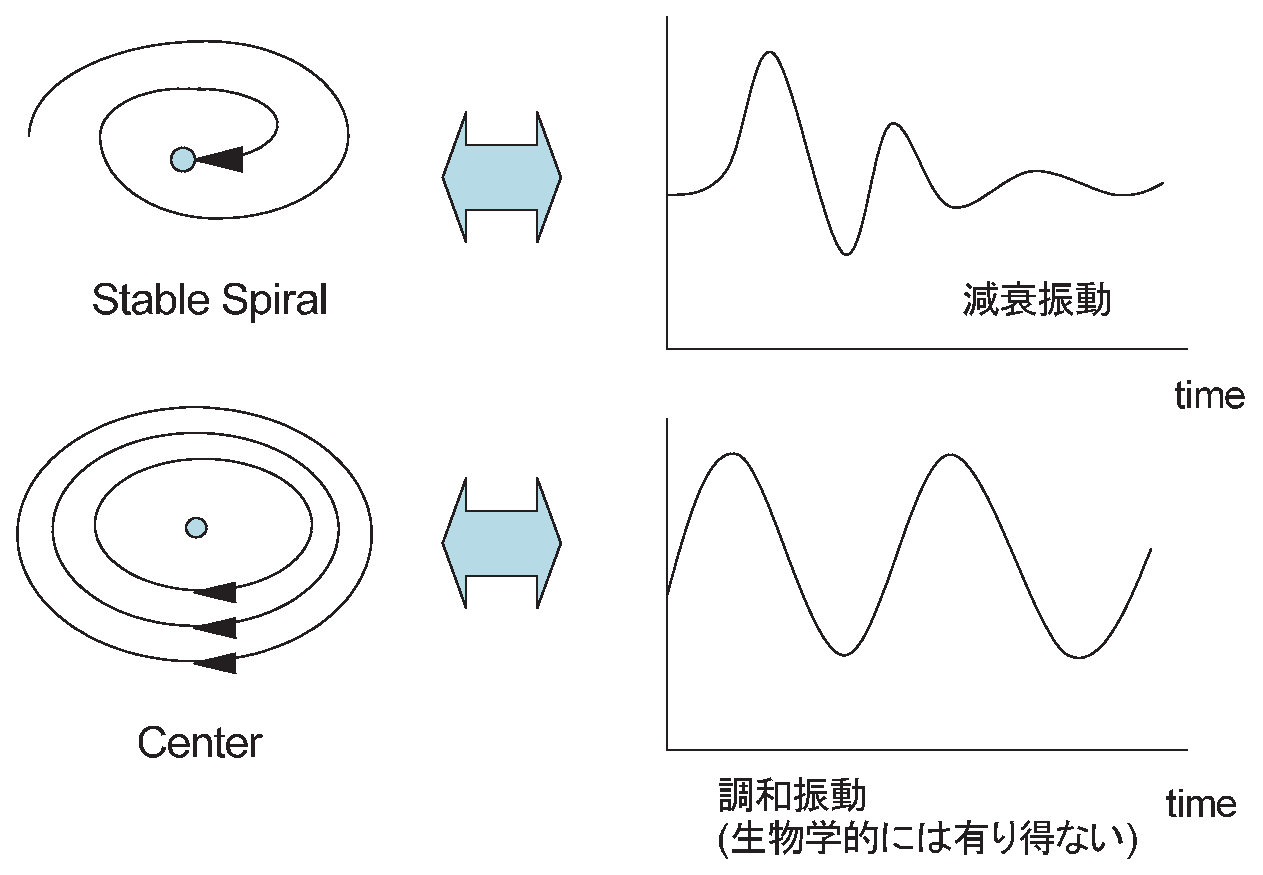
\includegraphics[height=6cm]{../Bifurcation/img/spiral_stability.eps}
        \caption{複素固有値を含む場合の固定点の分類。(左)それぞれの固定点近傍におけるベクトル場の特徴。実部の符号によって安定性を判別する。(右)時系列の特徴。}
        \label{fig:08bsysbio} \end{figure}


\paragraph{固有値の正負・虚実の判別法}
ヤコビ行列が2行2列の場合、下記のようにすると固有方程式を解かずに固有値の符号を知ることができます。ヤコビ行列を

\[{\bf J} =
\left(
\begin{array}{rr}
a& b\\
c& d\\
\end{array}
\right)
\]

とおくと、固有方程式は\(\lambda^2-(a+d)\lambda+(ad-bc)=0\)となります。この固有方程式の2つの解を\(\lambda_1\) 、\(\lambda_2\)とすると、2次方程式の解と係数の関係から、

\[
\begin{array}{lclclcl}
\tau & = & \lambda_1 + \lambda_2 & = & a + d & = & {\rm tr}({\bf J})\\
\Delta & = &\lambda_1 \lambda_2 & = & ad - bc & = & \det({\bf J})\\
\end{array}
\]

と書くことができます。\(\Delta\)の正負から、2つ固有値(の実部)が同符号であるか判定でき、その符号が正負どちらなのかは\(\tau\)の正負に対応します。また、\(\tau^2 -4\Delta\)の正負からは固有値が実数・複素数のどちらになるかを判定できます。


\paragraph{演習4:  Griffithモデルにおける固定点の分類}
ヤコビ行列の固有値の符号を調べ、Griffith モデルに現れる固定点を分類しなさい。

\subsection{分岐}
\paragraph{分岐(bifurcation)} パラメータの変化により、固定点の数や種類が変わること。Griffith モデルはパラメータの値によって、固定点の数、安定性が変わるSaddle-Node分岐を示します。

\paragraph{演習5:  Griffithモデルにおける分岐}
\(ab < \displaystyle\frac{1}{2}\)、\(ab=\displaystyle\frac{1}{2}\) 、\(ab > \displaystyle\frac{1}{2}\) の3つの場合についてベクトル場を描きなさい。固定点の個数、性質はどのように3つの場合でどのように異なっているか。


\section{Hopf(ホップ)分岐}
%\documentclass[a4paper,11pt]{jsarticle}
%\usepackage{graphicx}
%\usepackage{ascmac}
%\usepackage{url}

\def\演習問題#1{{\flushleft\underline{\bf 演習問題~#1}}}

%\begin{document}
\subsection{Sel'kov モデル: 振動現象}
\indent 比較的早くから見つかっていた生物リズムとして、出芽酵母解糖系に
おける物質濃度の振動があります。Sel'kovは1968年に図\ref{fig:09sysbio}
に示すモデルを提案し、解糖系の流束に影響力を持つ酵素であ
るphosphofructokinase(PFK)周辺のフィードバック・ループが振動子の核心で
あると主張しました。以降、このSel'kovモデルは生物リズムを説明する最もシ
ンプルな模型として多くの論文や教科書で取り上げられています。ここで
はSel'kovモデルを通じて振動現象を説明する数理を学びます。

\begin{figure}[ht]
        \centering 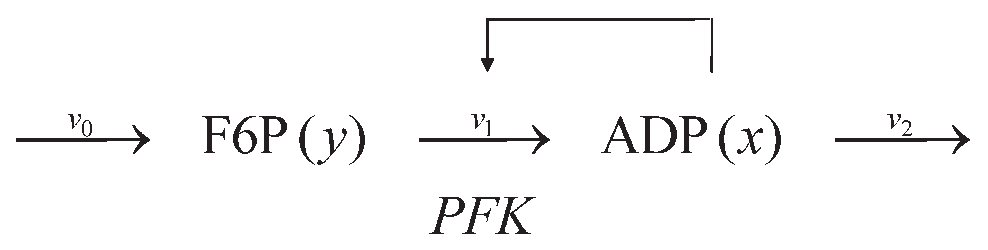
\includegraphics[height=1.5cm]{../Bifurcation/img/selkov_model.eps}
        \caption{Sel'kovモデル。ADPがPFKを活性化することによる正のフィードバック・ループを持つ。}
        \label{fig:09sysbio} \end{figure}

連立微分方程式で図\ref{fig:09sysbio} を表現したものを次に示します。

\[
\left\{
\begin{array}{lclclll}
\dot x & = & -x+ay+x^2 y\\
\dot y & = & b-ay-x^2y\\
\end{array}
\right.\]

ただし、\(x\)はADP、\(y\)はF6Pの存在量です。

\paragraph{リミットサイクル(limit cycle)} 相平面中にできる閉曲線。非線形振動の軌跡に相当します。
Center周囲には同心円状に閉軌道が存在する(図\ref{fig:08bsysbio})のに対し、リミットサイクルの周辺には
閉軌道は存在しません(図\ref{fig:09sysbio}右)。固有値を\(\lambda = a+bi\)とおいたとき、振動の周期はおおよそ\(\displaystyle\frac{2\pi}{b}\)となります。実習課題(3)で描いた概日時計モデルの解軌跡もリミットサイクルです。

\paragraph{Hopf 分岐 (Hopf bifurcation)}
振動現象ときわめて密接な関係にある分岐です。共役な複素固有値対が複素平面の虚軸を左から右に横切るとき(すなわち実部が負から正になるとき)、Stable spiralがUnstable spiralに変化することを指します。{\bf Hopf分岐が存在する場合、Unstable node の周囲にはリミットサイクルが存在することが保証されています。}よってHopf分岐により、系が定常状態から振動状態へとその挙動を変えます。
細胞内における分子濃度の振動現象のほとんどは Hopf 分岐で説明できます。

\begin{figure}[ht]
        \centering 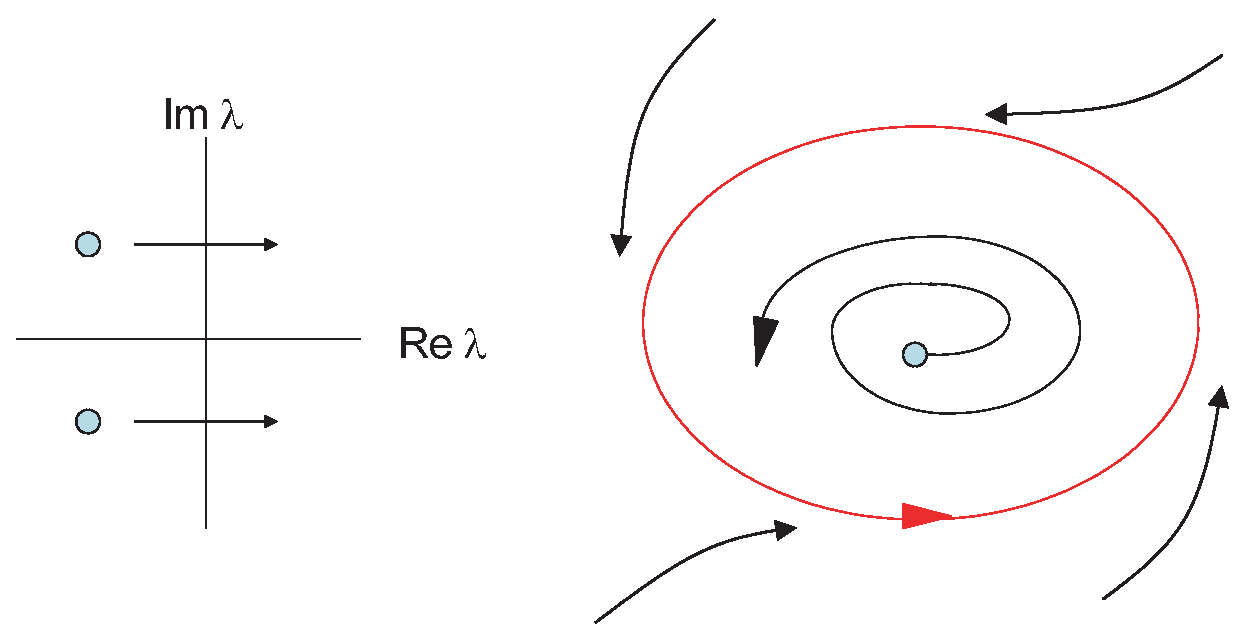
\includegraphics[height=6cm]{../Bifurcation/img/hopf_limitcycle.eps}
        \caption{(左)共役な複素固有値対が虚軸を左から右に横切るとき、Stable spiralがUnstable spiralに変化する。(右)これに伴い、Unstable spiral を取り巻くようにリミットサイクル(赤で描いた閉軌道)が生じる。}
        \label{fig:10sysbio} \end{figure}


\subsection{演習: Sel'kov モデルの解析}
\begin{enumerate}
\item Sel'kov モデルのヌルクラインを相平面上に描きなさい。
\item 「1」の結果にベクトル場の概略を描き加え、固定点がSpiralになると予想できることを確かめなさい。
\item Sel'kov モデルを線形化し、ヤコビ行列を求めなさい。
\item 2つの固有値の実部が同符号であることを確認しなさい(ヒント: \(\Delta\)の正負を調べる)。
\item Sel'kov モデルの固定点が Stable Spiral から Unstable Spiral へと変化するときに パラメータ\(a\)、\(b\)の間に成り立つ関係式を求めなさい(ヒント: \(\tau\)=0となる条件を調べる。理由はなぜか?)。
\item 「5」で求めた式に相当する曲線の概形を描きなさい。\(a\)、\(b\)をそれぞれ横軸、縦軸とすること。曲線を境に、どちら側がStableもしくはUnstableなのかも記入しなさい。
\end{enumerate}



\section{Pitchfork(熊手型)分岐}
\subsection{Toggle switch}
ボストン大学Collins lab.のGardnerらは、互いに抑制し合う遺伝子から成る人工遺伝子回路(図\ref{fig:11sysbio})を構築し、大腸菌細胞内で双安定スイッチ(toggle switch)として動作させることに成功しました。同じように双安定性を示す Griffith モデルが Saddle-Node 分岐を内包していたのとは異なり、Toggle switch は1個もしくは3個の固定点を持つ Pitchfork 分岐を起こします。

\begin{figure}[ht]
        \centering \includegraphics[height=3cm]{../Bifurcation/img/toggleswitch.epsi}
        \caption{GardnerらのToggle switch型遺伝子回路。2つのリプレッサーが、互いを抑制し合う。}
        \label{fig:11sysbio} \end{figure}

連立微分方程式で図\ref{fig:11sysbio} を表現したものを次に示します。

\[
\left\{
\begin{array}{lcl}
\dot x & = & \displaystyle\frac{a}{1+y^2} - x\\
\dot y & = & \displaystyle\frac{a}{1+x^2} - y\\
\end{array}
\right.
\]

式の形を見ると、\(x\)と\(y\)を置換しても同じ式になることがわかります。Pitchfork分岐はこのように対称性をもつ系に生じる分岐です(図\ref{fig:12sysbio})。

\begin{figure}[ht]
        \centering \includegraphics[height=3cm]{../Bifurcation/img/pitchfork.epsi}
        \caption{Pitchfork分岐の際の固定点のy座標の変化。分岐点を境に、固定点が1個から3個に増える。全体の形状が熊手(pitchfork)に似ているのが命名の由来。}
        \label{fig:12sysbio} \end{figure}


\subsection{演習: Toggle switch モデルの解析}
\begin{enumerate}
\item Toggle switch モデルのヌルクラインを相平面上に描きなさい。固定点の数は\(a\)の値によって1個または3個になりますが、どちらの場合でも構いません。
\item 「1」の結果にベクトル場の概略を描き加え、固定点が1個の場合はStable Nodeに、3個の場合はStable Node 2個とUnstable Node 1個になると予想できることを確かめなさい。
\item \(y\)についてのヌルクラインの式を\(x\)についてのヌルクラインの式に代入し、固定点の\(x\)座標が\(x^5-ax^4+2x^3-2ax^2+(1+a^2)x-a=0\)を満たすことを示しなさい。
\item 「3」で示した固定点\(x\)座標に関する条件式\(x^5-ax^4+2x^3-2ax^2+(1+a^2)x-a=0\)が\((x^3+x-a)(x^2-ax+1)=0\)と因数分解できることを確認しなさい。
\item 一般に、\(x^3+ax+b=0\) の形をした3次方程式の解の性質は、判別式\(D=-4a^3-27b^2\)で予測することができる。\(D>0\)ならば3つの実数解、\(D=0\)ならば重解、\(D<0\)ならば1つの実数解と2つの虚数解を持つ。因数分解によって生じた\(x^3+x-a\)について、\(x^3+x-a=0\)について1つの実数解と2つの虚数解があることを確認しなさい。
\item 2次方程式の部分 \(x^2-ax+1\) の解の判別式を求め、\(a=2\)を境に固定点が1個から3個に変化することを確認しなさい。
\item \(a>2\)のとき、2次方程式の部分 \(x^2-ax+1\) から求まる固定点について、ヤコビ行列の2つの固有値がともに負となることを確認しなさい(ヒント: \(\Delta\)の正負を調べる)
\end{enumerate}

\section{Further reading}
\noindent Strogatz, S.H, “Nonlinear dynamics and chaos”, Perseus Books Publishing, 1994. (ISBN 0-7382-0453-6)\\
(バイオロジストにとって最良の非線形力学系教科書。Borisuk and Tyson (1998)の背景知識学習にも最適。)\\

\noindent Fall, C.P., Marland, E.S., Wagner, J.M. and Tyson, J.J. “Computational cell biology”, Springer, 2002. (ISBN 0-387-95369-8)\\
(Bendixsonの基準など、振動を起こす系の必要十分条件に関する記述がわかりやすい。)\\

\noindent Borisuk, M.T. and Tyson, J.J., “Bifurcation analysis of a model of mitotic control in frog eggs”, J. Theor. Biol. 195:69-85, 1998.\\
(アフリカツメガエルの卵における細胞周期調節に関するモデル解析。ありとあらゆる分岐が登場するので、ケーススタディに最適。)\\

\noindent Griffith, J.S. Mathematics of cellular control processes. II. Positive feedback to one gene. J. Theor. Biol. 20, 209-16, 1668.\\
(Griffithモデルの初出論文。)\\

\noindent Sel'kov, E.E., Self-oscillations in glycolysis. 1. A simple kinetic model. Eur J Biochem. 4(1):79-86, 1968.\\
(Sel'kov モデルの初出論文。)\\

\noindent Gardner, T.S., Cantor, C.R. and Collins, J.J., Construction of a genetic toggle switch in Escherichia coli., Nature 403(6767):339-42, 2000.\\
(Toggle switch の初出論文。)\\

%\section{Poincar\'{e}-Bendixsonの定理}
%\section{Bendixsonの基準}

%\end{document}
